\chapter{Analysis}


\null\qquad After the set of parallelisability metrics has been devised and proposed (see chapter \ref{metrics}) and a working framework for metrics research and analysis has been implemented and set (chapter \ref{ppar-tool} describes developed PPar tool), software source code parallelisability metric values can be gathered and analysed. \newline
\null\qquad Figure \ref{analysis-data-table} below presents the data, used for analysis. This data has been extracted from NAS parallel benchmarks (see chapter \ref{benchmarks}) and transformed into tabular format. This data is, essentially, a set of loops found in NAS benchmarks. For every single loop a set of metrics (loop features) has been computed. All loops have passed through Intel C/C++ compiler parallelisability analyses and have been classified (labelled) as parallelizible or not. ICC compiler plays a role of expert in this project. The table contains around 1400 loops with and 13-dimensional feature vector for each.  

\begin{figure}[htb]
	\centering
	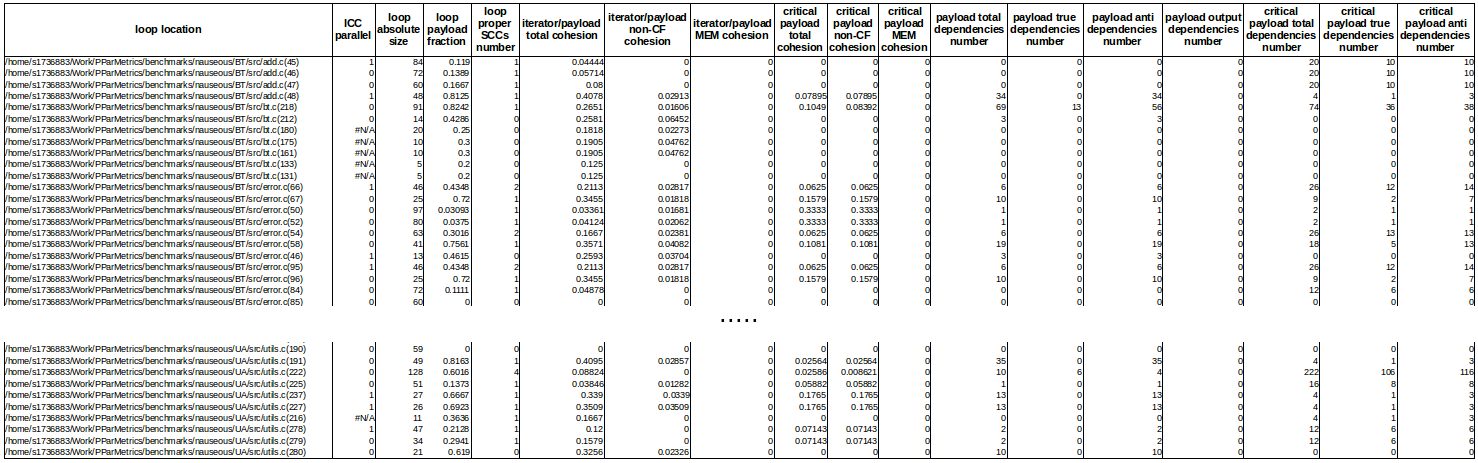
\includegraphics[width=\linewidth]{figs/metrics-table.png}
	\caption{Analysis input table with computed metrics and ICC parallelizability classification labels.}
	\label{analysis-data-table}
\end{figure}

\qquad This chapter describes analysis approaches and presents findings in the report. First, the collected data has been visualized to see any obvious correlations between loop parallelisability and metric values. Section \ref{analysis-data-interpretation-and-visualization} provides data interpretation and visualizations. Section \ref{analysis-manual-analysis} contains some insights into analysis results. Then, statistical analysis techniques have been applied to the data. Loop metrics have been viewed as machine learning features in the context of loop parallelisability classification problem. Standard state-of-the (such as Support Vector Machines (SVM), desicion trees, etc) machine learning techniques have been applied to the data and all prediction errors have been compared agains random predictor. Section \ref{analysis-statistical-analysis} presents a report on this. \newline
\null\qquad There has already been an attempt to apply statistical analysis techniques to see how software quality metrics, such as cyclomatic complexity \ref{background-cyclomatic-complexity} and Halstead's software science measures \ref{background-halsteads-measures} behave on Mozilla Firefox browser and LLVM compiler components library open source codes \cite{source-code-quality-classification-paper}. Authors applied k-means clustering and got 3 clusters of software quality metric values for subroutines. But there were no classifications attached to the input data and no correlations have been examined. There could easily be subroutines of different software quality grades in the same cluster. \newline

\section{Analyses preparation phase}
\label{analysis-preparation-phase}
\qquad As it turned out, there are some outliers in the collected data that distort the final result. 

\section{Data interpretation and visualization}
\label{analysis-data-interpretation-and-visualization}
\qquad The first step in the analysis of collected loop metrics and parallelisability properties is to visualize the data and manually check for existent data patterns and correlations. Python packages pandas \cite{python-lib-pandas} and matplotlib \cite{python-matplotlib} have been used for the task. 

\section{Data clustering analysis}
\label{analysis-data-clustering-analysis}

\subsection{Combined metrics data visualization}
\label{analysis-data-clustering-analysis}
\qquad This section describes an attempt to conduct structural data analysis and identify separate clusters in the data. Since loops are represented by 13-dimensional vectors, direct dataset visualization is unfeasible. Principal Components Analysis (PCA) has been used to project the data onto 3-dimensional space and visualize it. Figure \ref{metrics-pca-13-to-3} provides an illustration of distribution of metric values on all loops. It is visible from the figure, that data values do not form any apparent clusters, but there are some areas of increased density though.
\begin{figure}[htb]
\centering
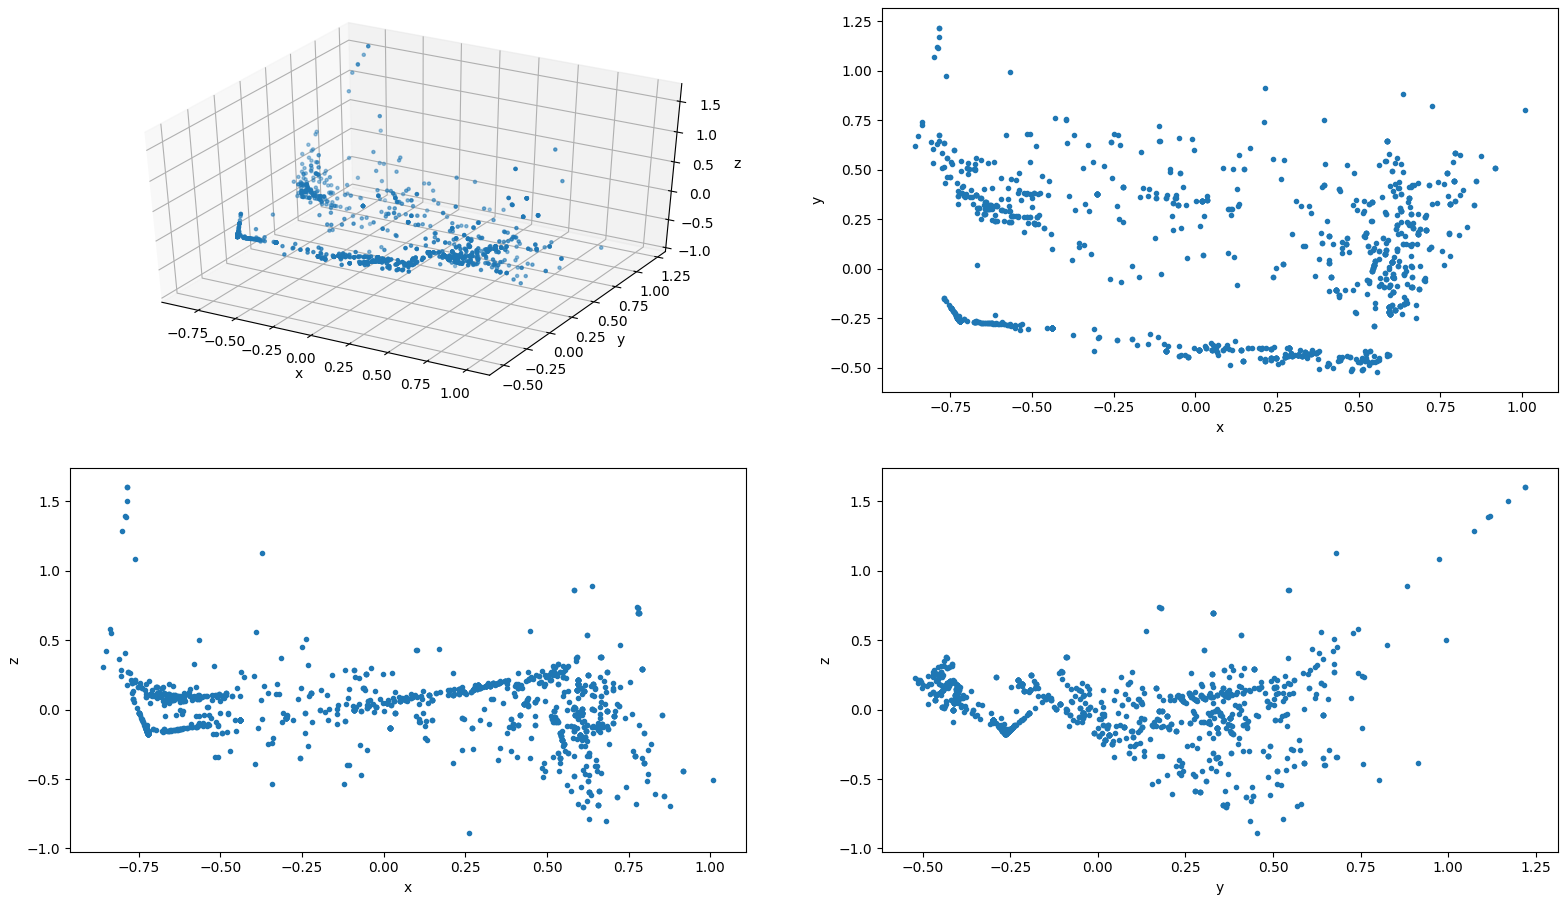
\includegraphics[width=\linewidth]{figs/metrics-pca-13-to-3.png}
\caption{Visualisation of loop metrics dataset (13-dimensional metric vectors have been projected onto 3d space thanks to PCA algorithm) - blue dots correspond to metric values on single loops.}
\label{metrics-pca-13-to-3}
\end{figure}

\qquad Metric dataset projection onto 2D plane looks alike XY projection of 3D PCA mapping (see figure \ref{metrics-pca-13-to-2}).

\section{Manual analysis}
\label{analysis-manual-analysis}

\subsection{The problem of proper SCCs number metric}
\qquad The proper SCCs number metric was described in section \ref{metrics-loop-proper-sccs-number}. Despite the fact, that the metric seems to directly represent parallelisability inhibiting parts of the payload, figures in ... show that ICC compiler sometimes fails to parallelise loops even with 0 metric value. Listing \ref{lst:metrics-loop-example-2} below, gives such example.

\begin{lstlisting}[caption={Non-parallelizible loop. Function call inside loop's body prevents ICC compiler from parallelizing it. Loop taken from EP NAS benchmark.}, captionpos=b, label=lst:metrics-loop-example-2]
for (i = 0; i < MK + 1; i++) {
	t2 = randlc(&t1, t1);
}
\end{lstlisting}

\begin{figure}[htb]
	\centering
	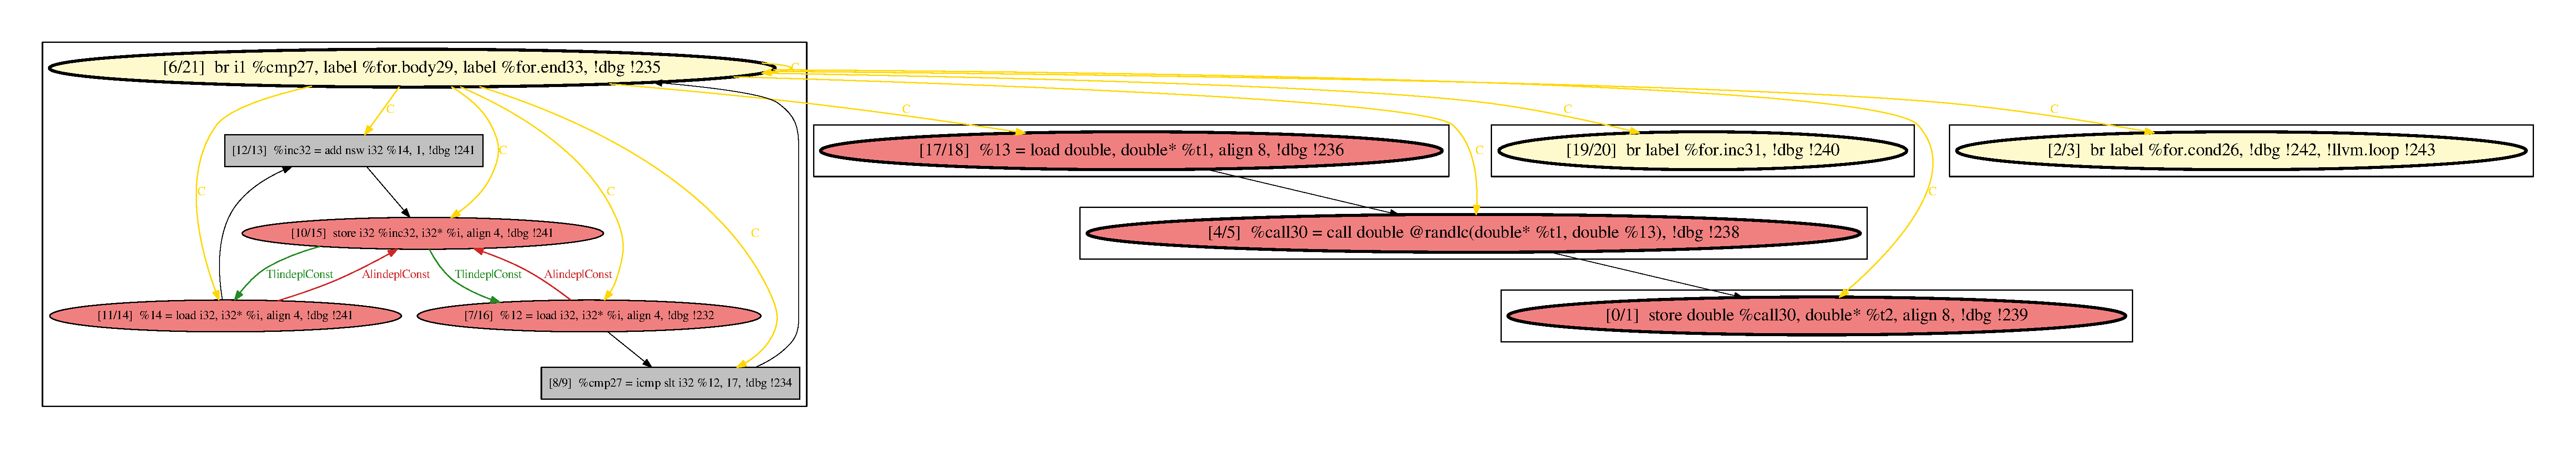
\includegraphics[width=\linewidth]{figs/metrics-example-loop-2-pdg.pdf}
	\caption{Program dependence graph (PDG) of the loop \ref{lst:metrics-loop-example-2}, as built and visualized by the PPar tool \ref{ppar-tool}.}
	\label{metrics-example-loop-2-pdg}
\end{figure}

\null\qquad Loop in the listing \ref{lst:metrics-loop-example-2} has a pretty simple PDG. There are no critical SCCs inside loop's payload. However, ICC compiler cannot parallelize this loop due to \textit{randlc} function call. Compiler has to be conservative and assume, that this function call introduces cross-iteration dependencies between iterations of the loop.\newline
\null\qquad This example exposes drawback of proper SCCs number metric. This metric only considers structural properties of PDG and does not examine the nature of instructions, constituting the loop. 


\section{Statistical analysis}
\label{analysis-statistical-analysis}
\qquad This section views loop parallelizability as a machine learning problem. Metrics represent features of loops. Intel C/C++ compiler gives an expert-opinion and labels (classifies) loops as parallelizible or not.
   
\qquad Statistical analysis of loop parallelisability metrics has been conducted with the help of pandas \cite{python-lib-pandas} and scikit-learn \cite{python-lib-scikit-learn} python packages. Detailed description of all algorithms, techniques and all underlying mathematical foundations can be found in the introduction to statistical analysis book \cite{statistical-learning-book}.

\subsection{K-Means clustering}

\qquad In this work k-means clustering techniques have been used as the first method of statistical analysis.




\subsection{SVM-based parallelisability analyzer}